\documentclass[a4paper]{article}
\usepackage[utf8]{inputenc}
\usepackage[russian]{babel}
\usepackage[T2]{fontenc}
\usepackage[warn]{mathtext}
\usepackage{graphicx}
\usepackage{amsmath}
\usepackage{floatflt}
\usepackage[left=20mm, top=20mm, right=20mm, bottom=20mm, footskip=10mm]{geometry}


\graphicspath{ {images/} }
\usepackage{multicol}
\setlength{\columnsep}{2cm}


\begin{document}

\begin{titlepage}
	\centering
	\vspace{5cm}
	{\scshape\LARGE Московский физико-технический институт \par}
	\vspace{4cm}
	{\scshape\Large Лабораторная работа \par}
	\vspace{1cm}
	{\huge\bfseries Дифракция света на периодических структурах (саморепродукция) \par}
	\vspace{1cm}
	\vfill
\begin{flushright}
	{\large выполнили студенты 653 группы ФФКЭ}\par
	\vspace{0.3cm}
	{\LARGE Карпова Татьяна} \par
		\vspace{0.3cm}
	{\LARGE Агафонов Владислав}
\end{flushright}
	

	\vfill

% Bottom of the page
	Долгопрудный, 2018 г.
\end{titlepage}

\section{Цель работы:}
Изучение явления саморепродукции и применение его к измерению параметров периодических структур.

\section{В работе используются:}
\begin{itemize}
    \item лазер
    \item кассета с сетками
    \item мира
    \item короткофокусная линза с микрометрическим винтом
    \item экран
    \item линейка
\end{itemize}

\section{Теоретические положения}
При дифракции на предмете с периодической структурой наблюдается явление саморепродукции: на некотором расстоянии от предмета вдоль направления распространения волны появляется изображение, которое потом периодически повторяется.  \par
Представим волну за периодическим объектом в виде суммы плоских волн разных направлений. Отдельные слагаемые плоские волны называют пространственными гармониками. Вдоль пути распространения волнового фронта на некотором расстоянии $z_0$ от предмета существует плоскость, где разность фазовых набегов любых пространственных гармоник (плоских волн идущих под углом $\theta$т к оси распространения), входящих в состав суперпозиции, кратна $2T$ В этой плоскости фазовые соотношения между всеми плоскими волнами, входящими в состав суперпозиции, такие же, что и в предметной плоскости. Поэтому в результате интерференции этих волн возникает изображение, тождественное исходному периодическому объекту. Все сказанное справедливо для любого расстояния $z_n$, кратного $z_0$. Для решетки с периодом $d$.
\begin{equation}
    z_n = \frac{2d^2}{\lambda}n
\end{equation}

Суть эксперимента по саморепродукции состоит в том, что дифрагированная на периодическом транспаранте (решетка, сетка) плоская монохроматическая волна лазера (лазерный пучок) воспроизводит изображение транспаранта без каких-либо оптических элементов.

    \begin{figure}[h]
    \centering
    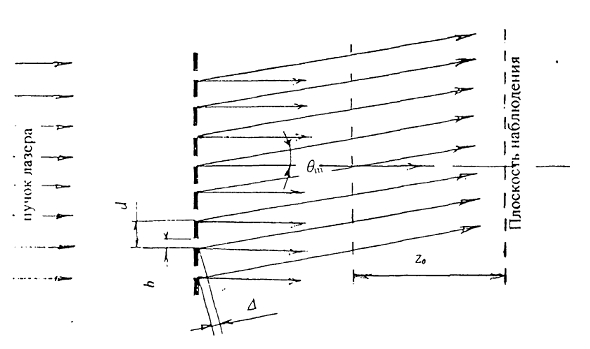
\includegraphics[width=15cm]{fig1.PNG}
    \caption{Дифракция лучей на сетке и возникновение саморепродуцированного изображения}
    \label{fig:vac}
\end{figure}

\section{Схема установки}

    \begin{figure}[h]
    \centering
    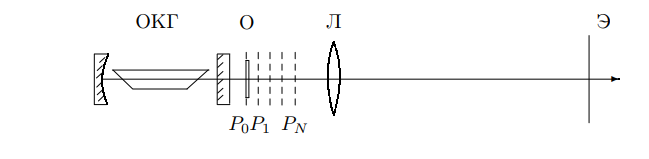
\includegraphics[width=15cm]{fig2.PNG}
    \caption{Схема лабораторной установки}
    \label{fig:vac}
\end{figure}

\section{Ход работы}

\subsection{Определение периода решёток по их пространственному спектру}

Измерим расстояние между соседними дифракционными максимумами и рассчитаем период каждой решётки:
    \begin{equation}
        d = \frac{\lambda L}{x},
    \end{equation}
    где $x$ - расстояние между соседними максимумами, $L$ - расстояние между решёткой и экраном, $\lambda$ - длина волны лазера. Результаты занесём в таблицу 1.

    \begin{table}[h]
    \centering
    \begin{center}
    \caption{Периоды решёток, метод 1}
    \end{center}
    \vspace{0.1cm}
    \label{tab:my_label}
    \begin{tabular}{ |p{2.5cm}||p{0.7cm}|p{0.7cm}|p{0.7cm}|p{0.7cm}|p{0.7cm}|}
 \hline
Номер решётки & 1 & 2 & 3 & 4 & 5\\
 \hline
 $d$, мм & 0.020 & 0.030 & 0.058 & 0.118 & 0.168\\

 \hline
 
\end{tabular}
\end{table}
    


\subsection{Определение периода решёток по изображению, увеличенного с помощью линзы}


Определим размеры клеток, полученных с помощью линзы, на экране (рассматриваем геометрическое изображение решётки) ($D$). Расстояние от линзы до сетки $a$, от линзы до экрана $b$, тогда период сетки считается по формуле 
    \begin{equation}
        d = D\frac{a}{b}
    \end{equation}
    Результаты измерения периода занесём в таблицу 2.


    \begin{table}[h]
    \centering
    \begin{center}
    \caption{Периоды решёток, метод 2}
    \end{center}
    \vspace{0.1cm}
    \label{tab:my_label}
    \begin{tabular}{ |p{2.5cm}||p{0.7cm}|p{0.7cm}|p{0.7cm}|p{0.7cm}|}
 \hline
Номер решётки & 1 & 2 & 3 & 4\\
 \hline
 $d$, мм & 0.028 & 0.054 & 0.132 & 0.156\\

 \hline
 
\end{tabular}
\end{table}

\subsection{Исследование эффекта саморепродукции с помощью сеток}

\begin{enumerate}
    \item Найдём координаты  $z_n$ плоскостей саморепродукции, построим график $z_n=f(n)$, коэффициенту наклона графика $k$ определим период решётки:
    \begin{equation}
    d = \sqrt{\frac{k \lambda}{2}}        
    \end{equation}
    
\begin{figure}[h]
\begin{center}
\begin{minipage}[h]{0.45\linewidth}
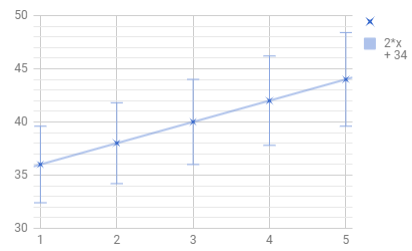
\includegraphics[width=1\linewidth]{g2.PNG}
\caption{Зависимость z(n), решётка 2} %% подпись к рисунку
\label{ris:experimoriginal} %% метка рисунка для ссылки на него
\end{minipage}
\hfill 
\begin{minipage}[h]{0.45\linewidth}
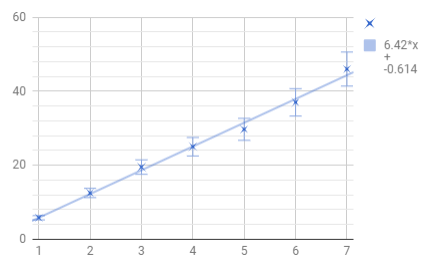
\includegraphics[width=1\linewidth]{g3.PNG}
\caption{Зависимость z(n), решётка 3}
\label{ris:experimcoded}
\end{minipage}
\end{center}
\end{figure}

\begin{figure}[h]
\begin{center}
\begin{minipage}[h]{0.45\linewidth}
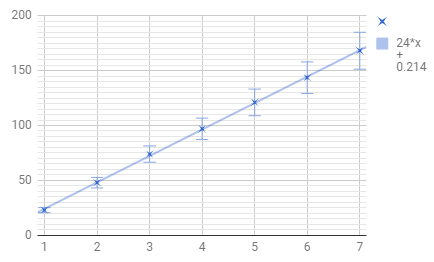
\includegraphics[width=1\linewidth]{g4.PNG}
\caption{Зависимость z(n), решётка 4} %% подпись к рисунку
\label{ris:experimoriginal} %% метка рисунка для ссылки на него
\end{minipage}
\hfill 
\begin{minipage}[h]{0.45\linewidth}
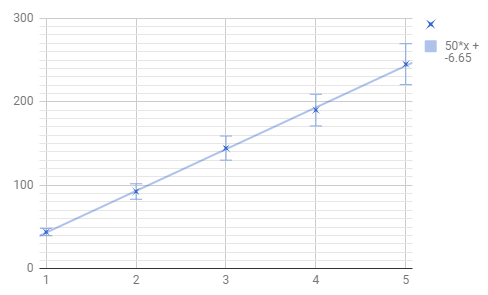
\includegraphics[width=1\linewidth]{g5.PNG}
\caption{Зависимость z(n), решётка 5}
\label{ris:experimcoded}
\end{minipage}
\end{center}
\end{figure}



    \begin{table}[h]
    \centering
    \begin{center}
    \caption{Периоды решёток, метод 3}
    \end{center}
    \vspace{0.1cm}
    \label{tab:my_label}
    \begin{tabular}{ |p{2.5cm}||p{0.7cm}|p{0.7cm}|p{0.7cm}|p{0.7cm}|}
 \hline
Номер решётки & 1 & 2 & 3 & 4\\
 \hline
 $d$, мм & 0.023 & 0.041 & 0.080 & 0.115\\

 \hline
 
\end{tabular}
\end{table}

\item Сведём результаты измерения периодов решёток тремя методами в единую таблицу 4



    \begin{table}[h]
    \centering
    \begin{center}
    \caption{Сравнение значений периодов, полученных разными способами}
    \end{center}
    \vspace{0.1cm}
    \label{tab:my_label}
    \begin{tabular}{ |p{2.5cm}||p{0.7cm}|p{0.7cm}|p{0.7cm}|p{0.7cm}|}
 \hline
Номер решётки & 1 & 2 & 3 & 4\\
 \hline
 $d$, мм & 0.030 & 0.058 & 0.118 & 0.168\\
\hline
 $d$, мм & 0.028 & 0.054 & 0.132 & 0.156\\
\hline
 $d$, мм & 0.023 & 0.041 & 0.080 & 0.115\\
\hline
 
\end{tabular}
\end{table}

Видим, что значения периодов, полученные при исследовании эффекта саморепродукции, отличаются в меньшую сторону примерно в 1,5 раза.
\end{enumerate}

\subsection{Исследование миры}

Установив миру на место кассеты, измерим период одного элемента сначала по саморепродукции, затем по увеличенному изображению и, наконец, по спектру. В таблицу 5 занесём эти результаты для миры с периодами 25 и 20.

\begin{figure}[h]
\begin{center}
\begin{minipage}[h]{0.45\linewidth}
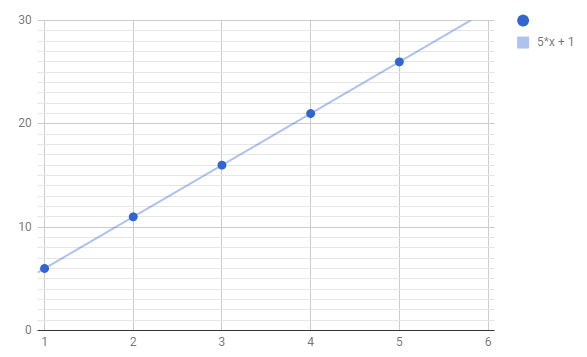
\includegraphics[width=1\linewidth]{m20.PNG}
\caption{Зависимость z(n), мира 20} %% подпись к рисунку
\label{ris:experimoriginal} %% метка рисунка для ссылки на него
\end{minipage}
\hfill 
\begin{minipage}[h]{0.45\linewidth}
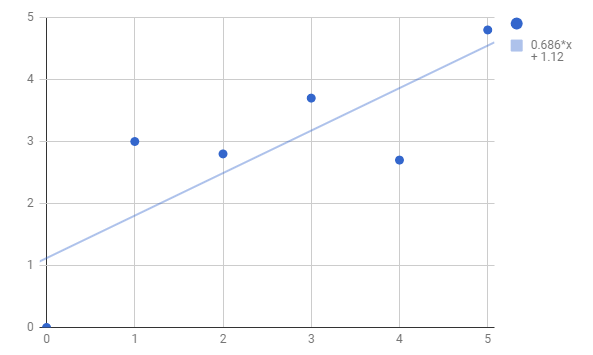
\includegraphics[width=1\linewidth]{m25.PNG}
\caption{Зависимость z(n), мира 25}
\label{ris:experimcoded}
\end{minipage}
\end{center}
\end{figure}

    \begin{table}[b]
    \centering
    \begin{center}
    \caption{Сравнение значений периодов мир, полученных разными способами}
    \end{center}
    \vspace{0.1cm}
    \label{tab:my_label}
    \begin{tabular}{ |p{3cm}||p{3cm}|p{3cm}|}
 \hline
 & Мира 20 & Мира 25\\
 \hline
 Спектр & 0.053 & 0.039 \\
\hline
 Линза & 0.047 & 0.07 \\
\hline
 Саморепродукция & 0.036 &  0.013\\
\hline

 
\end{tabular}
\end{table}


Непосредственно нами было проведено измерение миры-20, значения получились с меньшим разбросом.

\newpage

	\vspace{20cm}


\section{Вывод}

В работе изучено явление саморепродукции и его применение к измерению периодов решеток. Параметры данных периодических структур измерены двумя дополнительными методами (по спектру и по увеличенному изображению через линзу). Дополнительные методы измерения дали совпадающие по порядку результаты, а методом саморепродукции результаты уменьшены в 1,5 раза по сравнению с дополнительными измерениями. Результаты измерений и их сравнение представлены в таблицах выше. 

Также исследованы параметры элементов миры аналогичными методами. Результаты совпали по порядку величины.

\end{document}
